\section{Conservation}


\subsection{1D Conservation Laws}
We expect the following quantities to be conserved: mass h, momentum or mass velocity, $hu$ and $hv$, and
energy 0.5($hv^2$+$gh^2$). Potential vorticity is only looked at in the 2D solver. 
\newline

Invesigation of conservation laws in the 1D solver shows differences
between the conserved quantities. The solution array and time vector in the 1D solver define $U$ using
 a final index $x$, that is not physical $-$\textit{ghost point}, but is used for the periodic boundary 
 conditions. The mass is hypothetically guessed to be strictly conserved by the scheme, the momentum should also
 be strictly conserved by the scheme, unless there are reflections when the walls take some of the momentum. Lastly,
 the energy is of course physically conserved, but the inherent nature of the numerical scheme does not initially
capture this. Analysis shows energy conservation converges, which suggests after the intial transfer of potential energy
to kinetic energy produced by the initial conditions, the scheme is able to restore conservation. 
\newline


\begin{figure}[h!]
    \centering
    \begin{subfigure}[b]{0.312\textwidth}
        \centering
        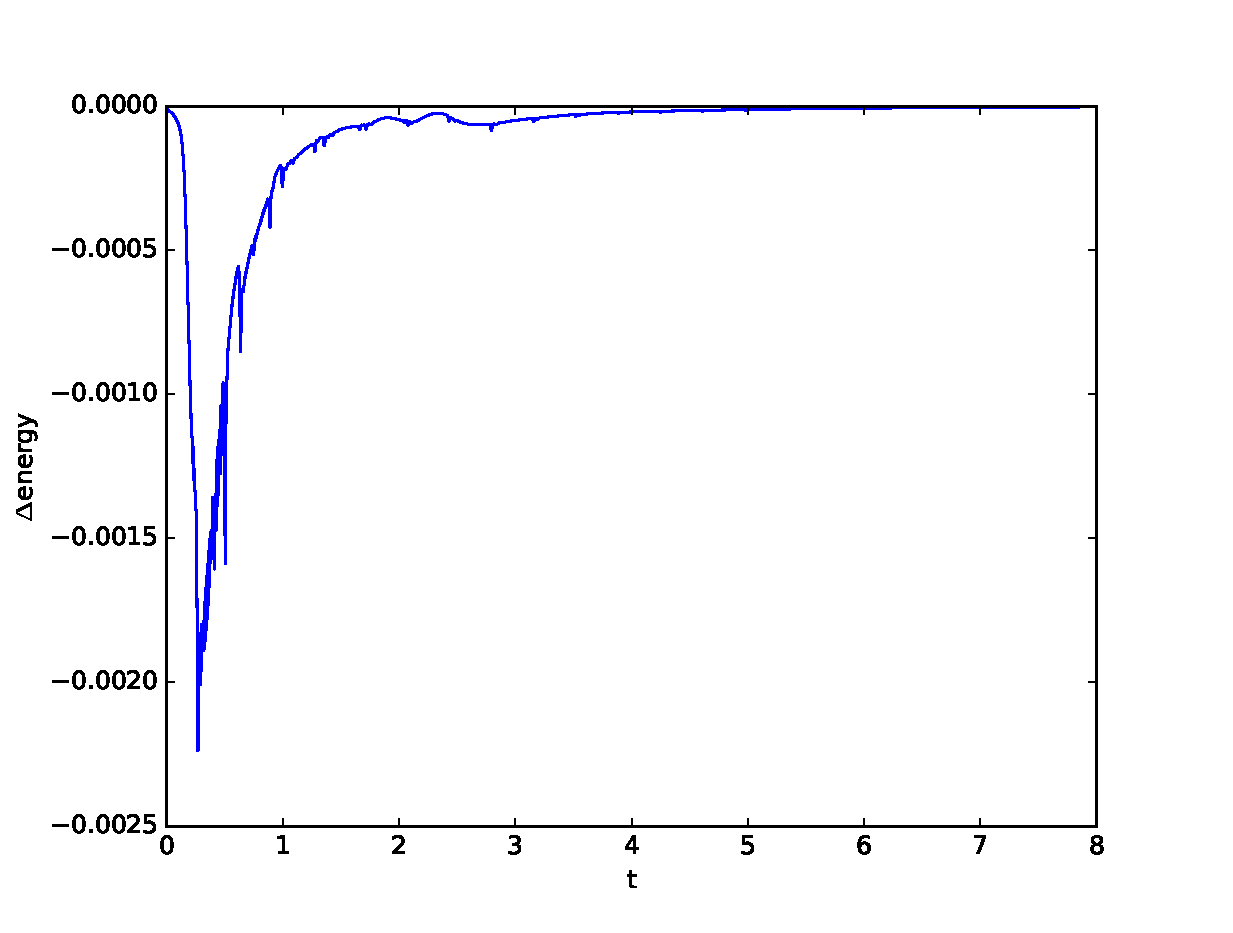
\includegraphics[width=\textwidth]{images/E1d.eps}\hfill
        \caption{Energy}
        \label{fig:Energy}
    \end{subfigure}
    \hfill
    \begin{subfigure}[b]{0.32\textwidth}
        \centering
        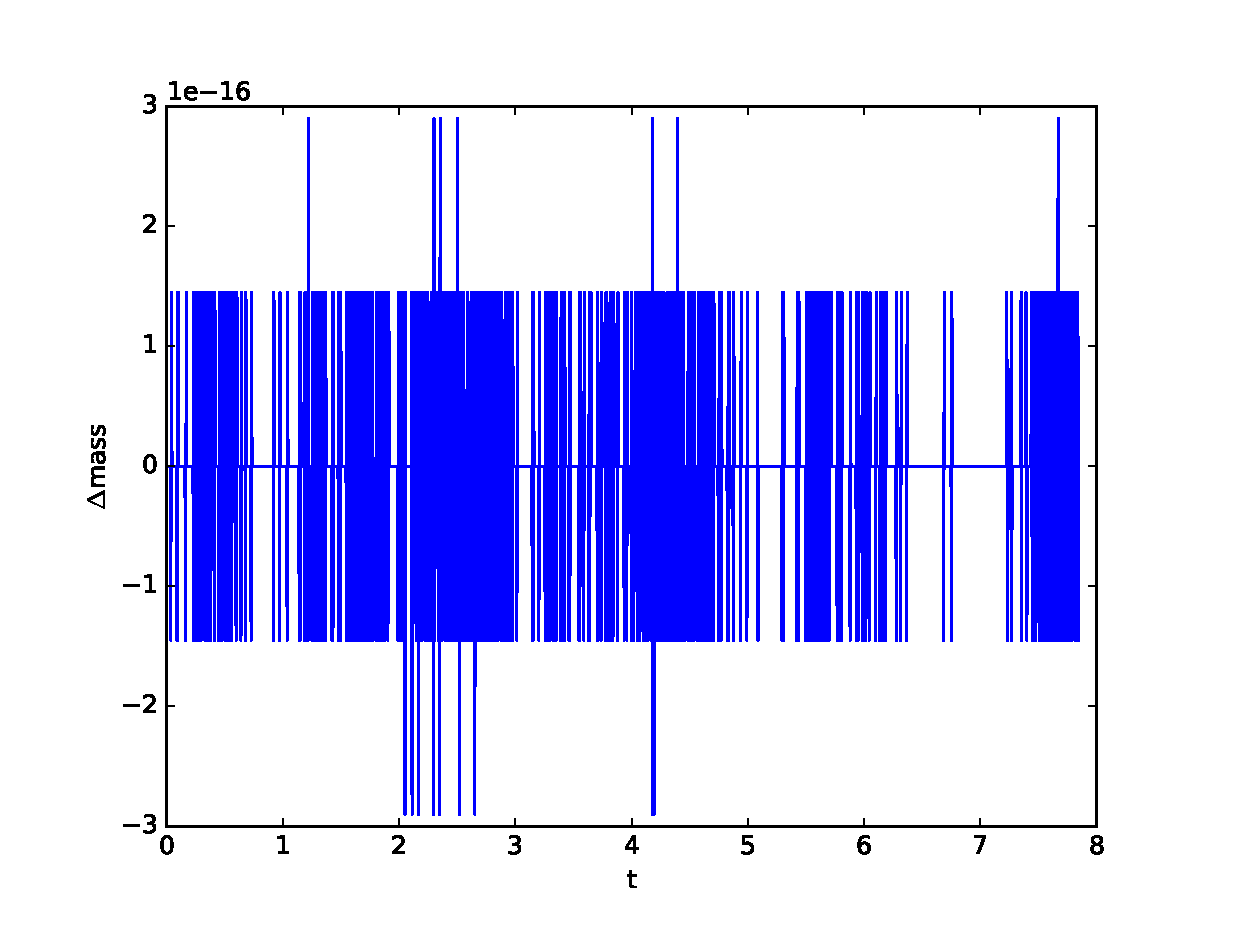
\includegraphics[width=\textwidth]{images/Ma1d.eps}\hfill
        \caption{Mass}
        \label{fig:Mass}
    \end{subfigure}
    \hfill
    \begin{subfigure}[b]{0.32\textwidth}
        \centering
        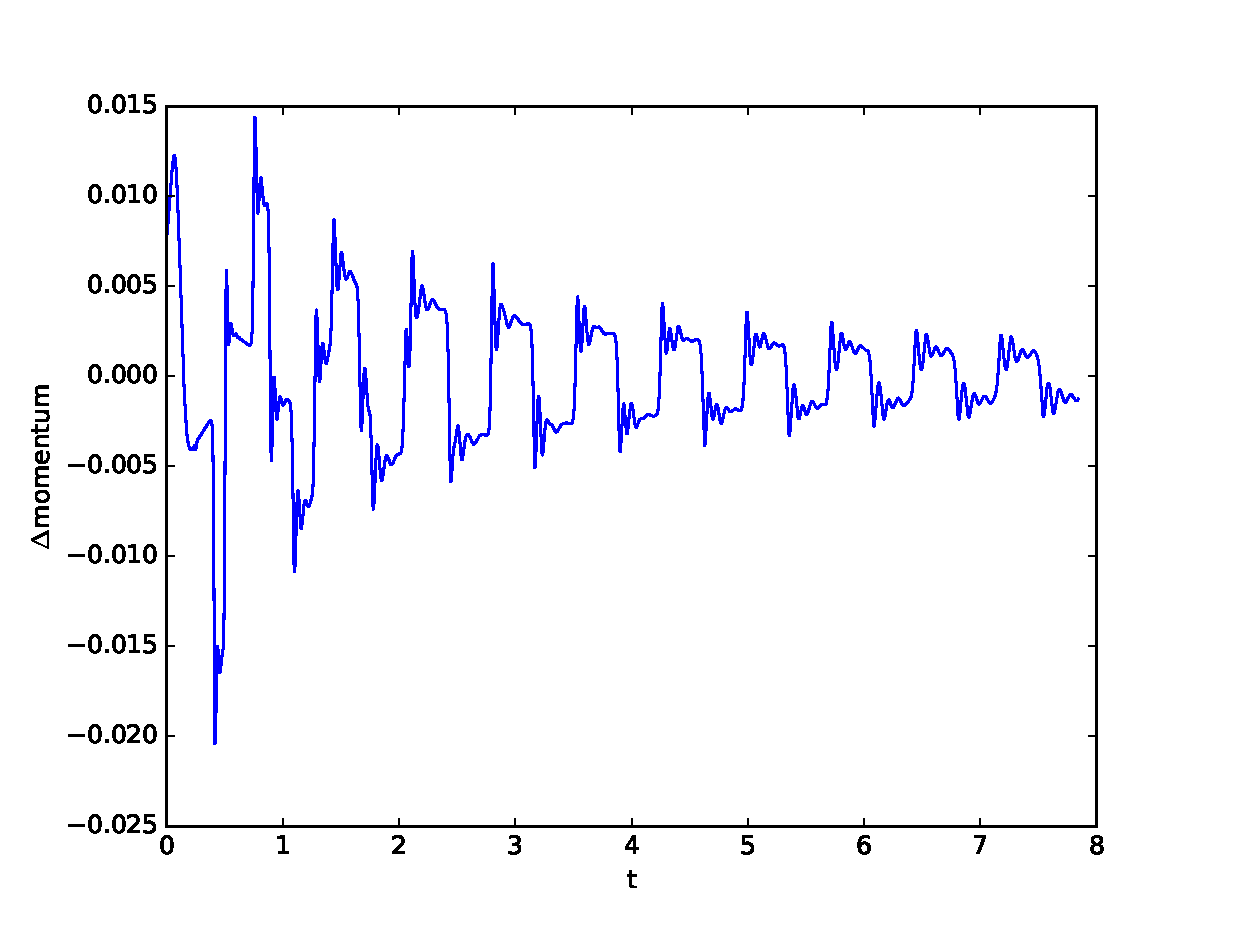
\includegraphics[width=\textwidth]{images/Mo1d.eps}\hfill
        \caption{Momentum}
        \label{Momentum}
    \end{subfigure}
    \caption{1D conservation plots.}
    \label{fig:three graphs}
\end{figure}







\begin{figure}[h!]
    \centering
    \begin{subfigure}[b]{0.46\textwidth}
        \centering
        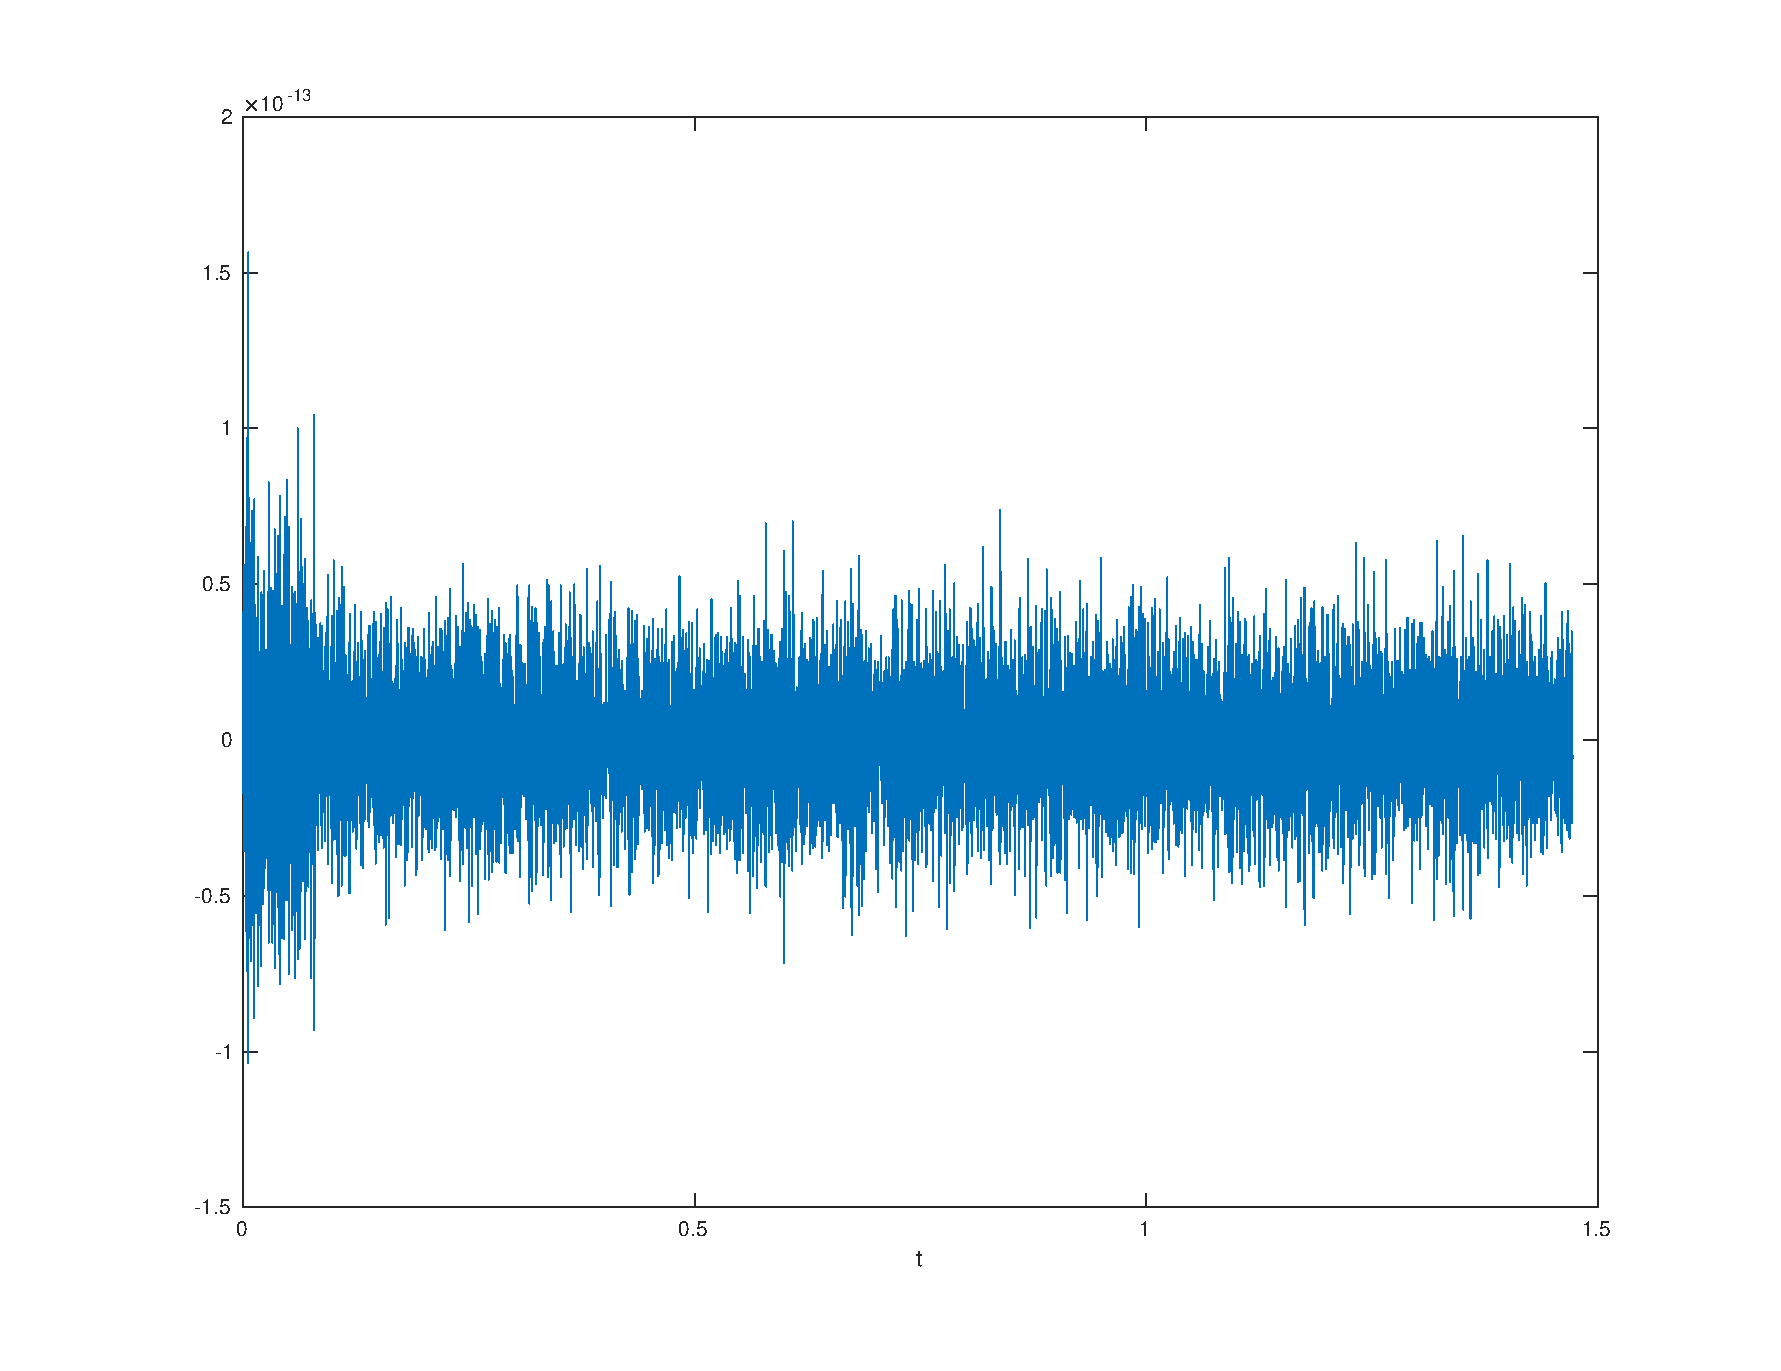
\includegraphics[width=\textwidth]{images/cons_mass.eps}\hfill
        \caption{Mass}
        \label{fig:Energy}
    \end{subfigure}
    \hfill
    \begin{subfigure}[b]{0.45\textwidth}
        \centering
        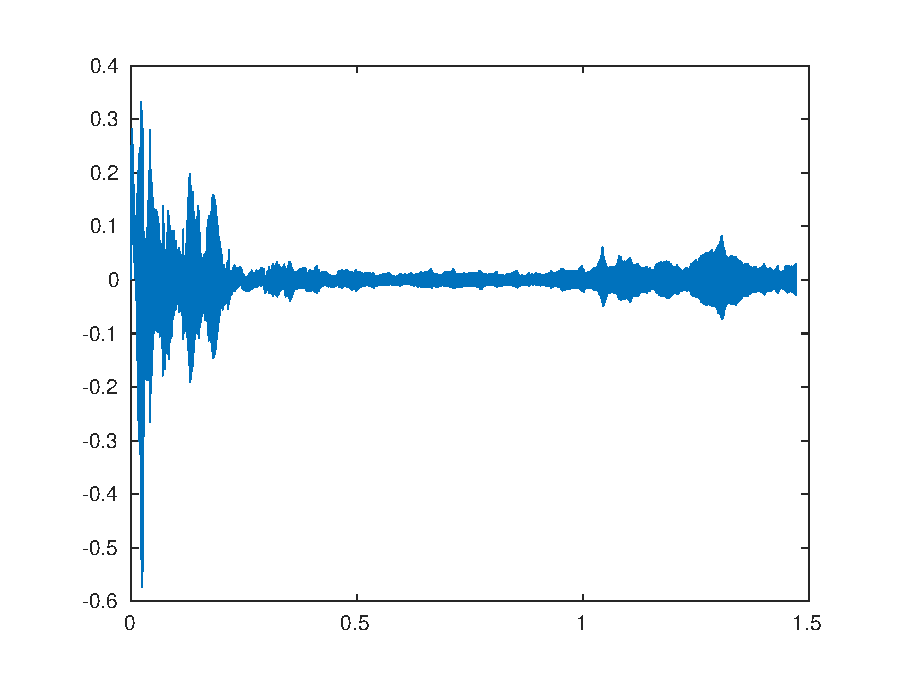
\includegraphics[width=\textwidth]{images/cons_energy.eps}\hfill
        \caption{Energy}
        \label{fig:Mass}
    \end{subfigure}
    \caption{2d conservation plots for mass and energy.}
    \label{fig:three graphs}
\end{figure}

\begin{figure}[h!]
    \centering
    \begin{subfigure}[b]{0.3\textwidth}
        \centering
        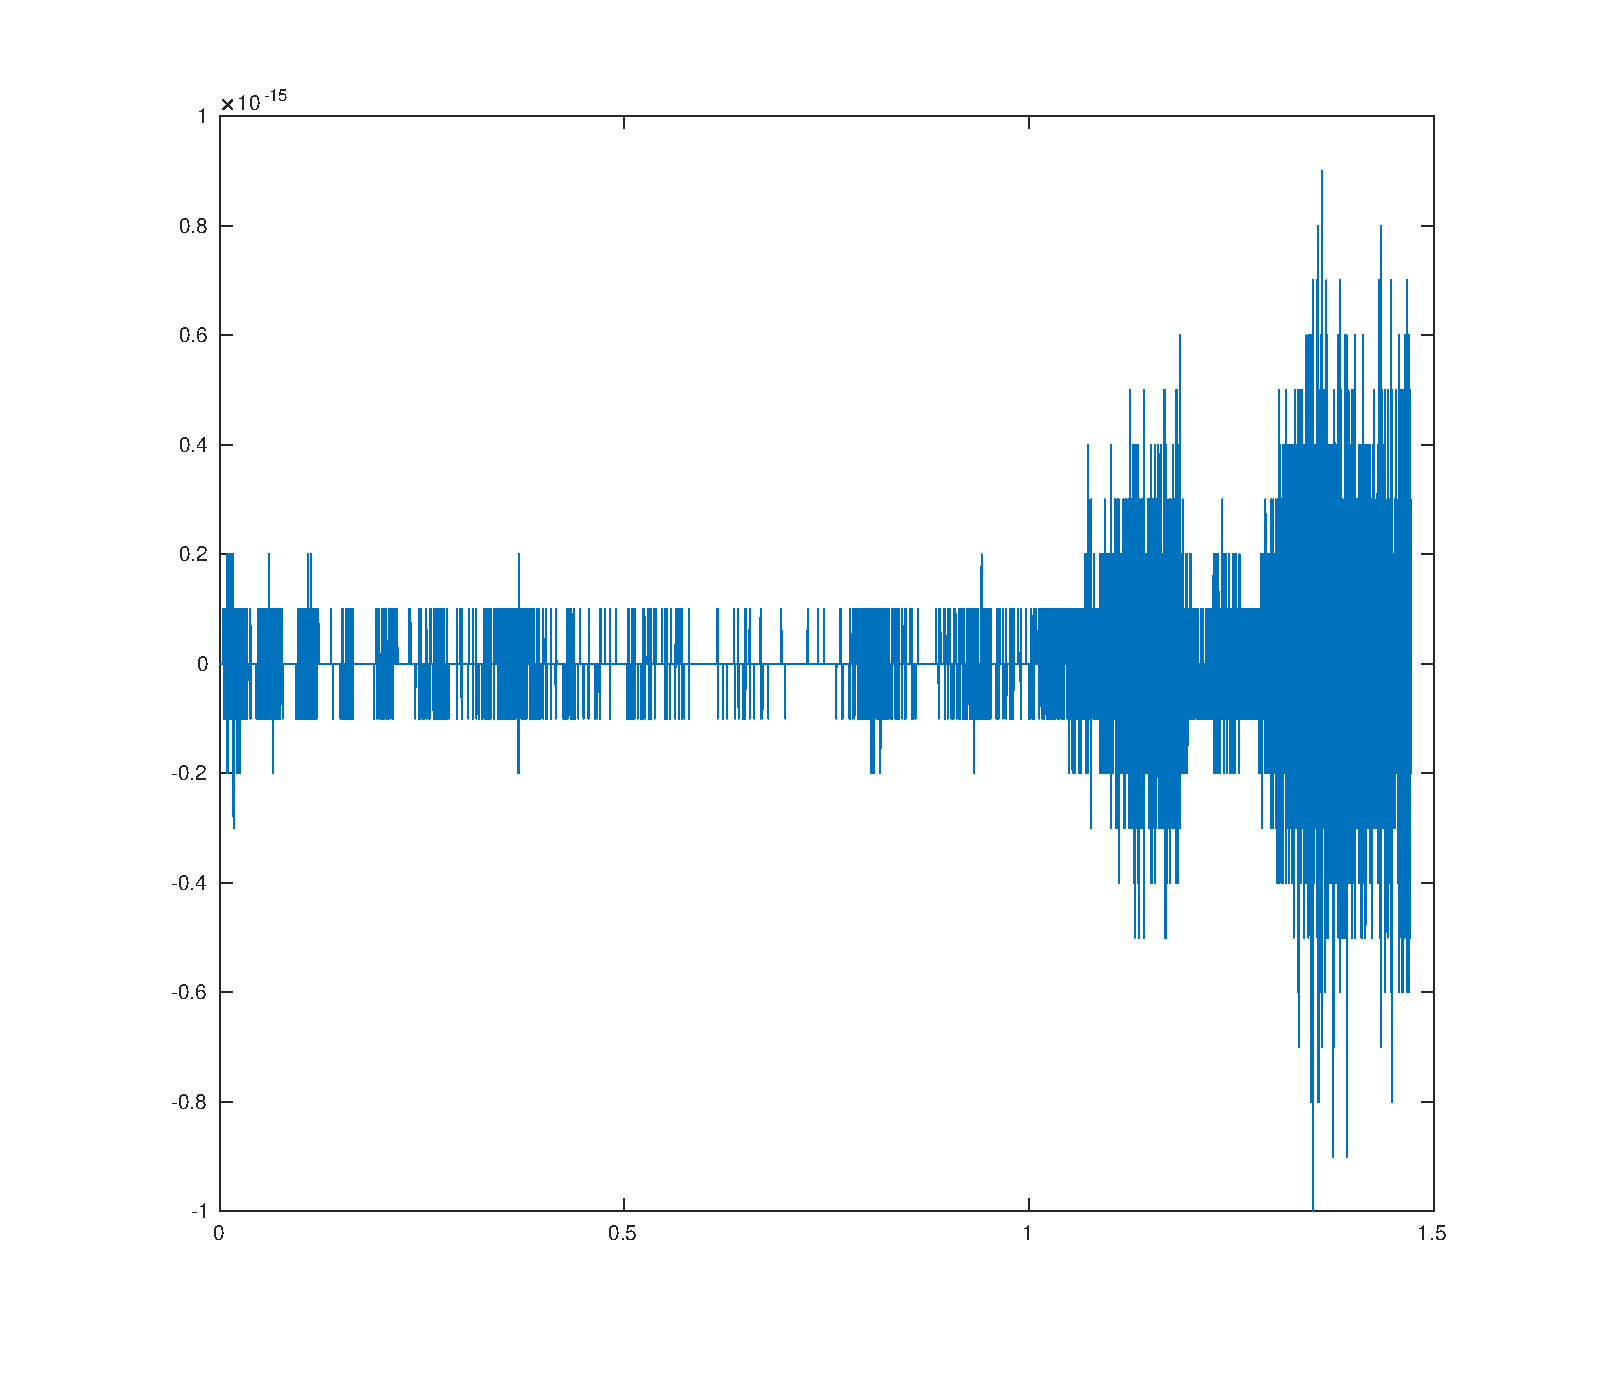
\includegraphics[width=\textwidth]{images/cons_momu.eps}\hfill
        \caption{u-momentum}
        \label{fig:mumu}
    \end{subfigure}
    \hfill
    \begin{subfigure}[b]{0.3\textwidth}
        \centering
        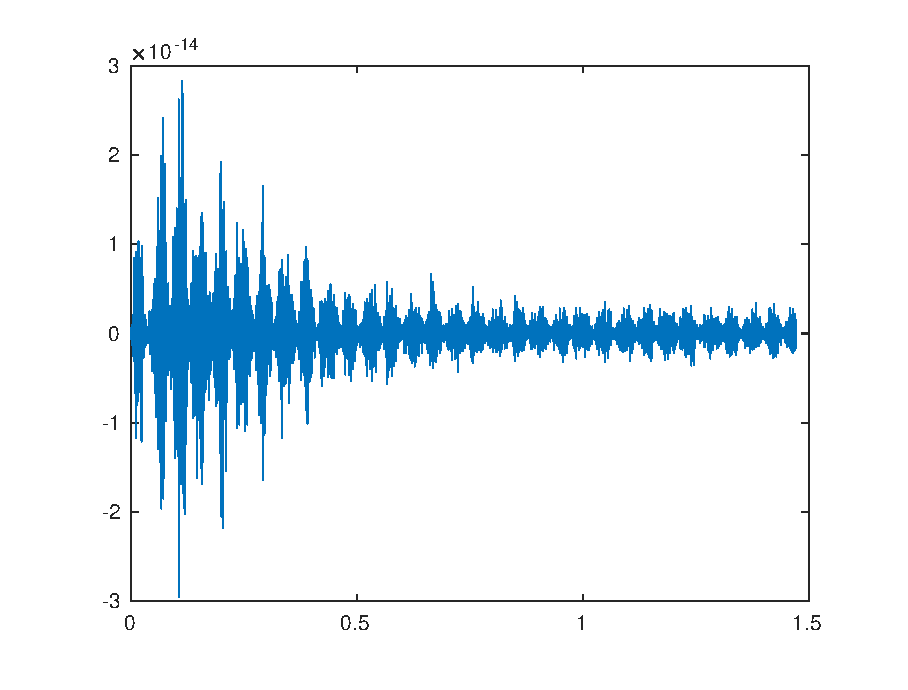
\includegraphics[width=\textwidth]{images/cons_momv.eps}\hfill
        \caption{v-momentum}
        \label{fig:momv}
    \end{subfigure}
    \hfill
    \begin{subfigure}[b]{0.3\textwidth}
        \centering
        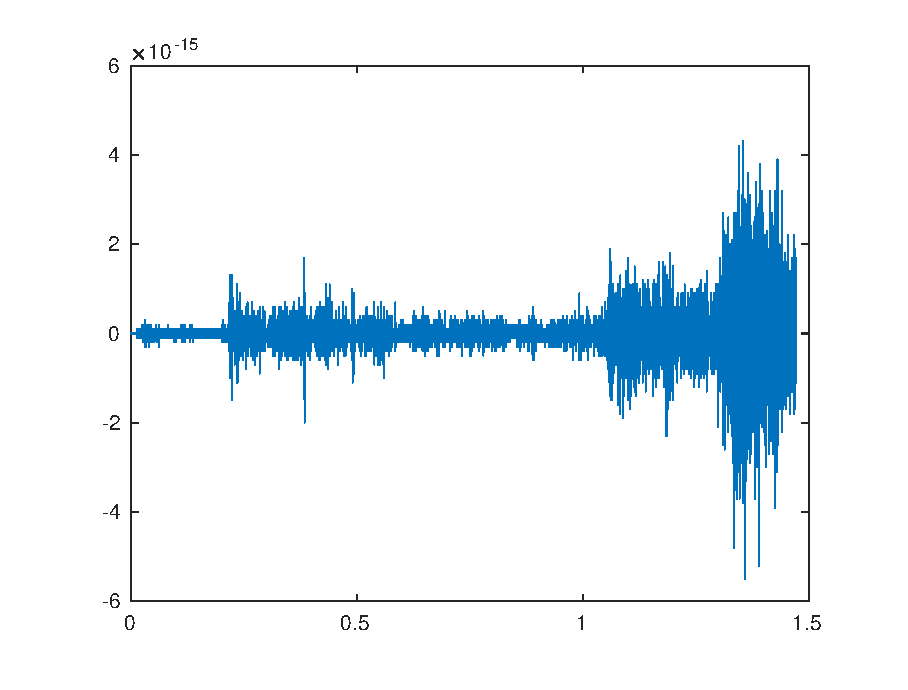
\includegraphics[width=\textwidth]{images/cons_vort.eps}\hfill
        \caption{vorticity}
        \label{fig:vort}
    \end{subfigure}
     \hfill
    \caption{2D Conservation plots.}
    \label{fig:three graphs}
\end{figure}



Lorem ipsum dolor sit amet, ad vix saperet mediocrem consetetur, ut admodum torquatos maiestatis est, 
no aeque singulis interpretaris sea. Ut paulo petentium eum, eum id malorum dignissim. Sed ex modus quodsi. 
Simul commodo scribentur ne has, mei ei dico interpretaris. Iriure tibique gloriatur vim an. Mea ea idque 
fabulas lucilius.

Vel timeam fuisset te. Duo ea nobis omnium pericula, sed discere scripserit ei, mea an illud dolore adolescens.
 Eu cum eligendi voluptatum, brute lobortis eam an, ea mei fastidii complectitur. An causae accusam pri. 
 In ius possit oportere.ges: